\chapter{Konzeption}

Um den \textit{SSD} und den \textit{YOLO} Objektdetektor miteinander vergleichbar zu machen und um deren Potential zum industriellen Einsatz zu bewerten, müssen konkrete Bewertungskriterien eingeführt werden. Anhand dieser Metriken werden die beiden Objektdetektoren auf einem Benchmark Datensatz initial verglichen, bevor der eigentliche Datensatz eingeführt wird. Dieser wird der Echtzeitumgebung entnommen. 

\section{Bewertungskriterien}

\subsection*{Präzision}

Um die Genauigkeit von Objektdetektoren zu messen, wird oft die Metrik \textit{mean Average Precision} (mAP) gewählt. Diese setzt sich aus zwei grundlegenden Größen zusammen (siehe Abbildung \ref{metrics}). 

\begin{figure}[ht]
	\begin{center}
		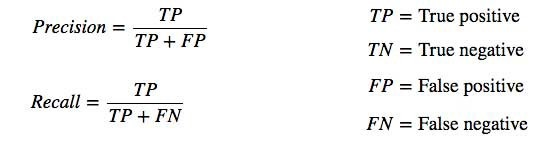
\includegraphics[width=10cm]{Bilder/metrics.png} 
		\caption[Precision und Recall Metrik]{Precision und Recall \cite{JonathanHui.20180307}}
		\label{metrics}
	\end{center}
\end{figure}

\textit{Precision} sagt also etwas über die Verlässlichkeit einer Klassifikation aus während \textit{Recall} Aussagen über die Erkennungsfähigkeit eines Objektdetektors trifft. Wichtig ist es hierbei anzumerken, dass mehrfach detektierte Objekte nur einmal als positiver Befund aufgefasst werden, die restlichen Detektionen gehen als \textit{False Positives} \cite{TarangShah.20180127}.

Die Klassifikation, ob eine Region das gewünschte Objekt enthält und demnach ein positiver Fall vorliegt, wird anhand des definierten \textit{IoU} Schwellwertes bestimmt. Dieser wird auch als \textit{confidence score} bezeichnet. Für den kompletten Datensatz werden nun für unterschiedliche \textit{confidence scores} jeweils \textit{Precision} und \textit{Recall} bestimmt und anschließend in einem Graphen aufgetragen. Meistens werden die \textit{confidence scores} so gewählt, sodass sich eine äquidistante Abstufung in den \textit{Recall} Werten ergibt \cite{TarangShah.20180127}. 

\begin{figure}[ht]
	\subfigure{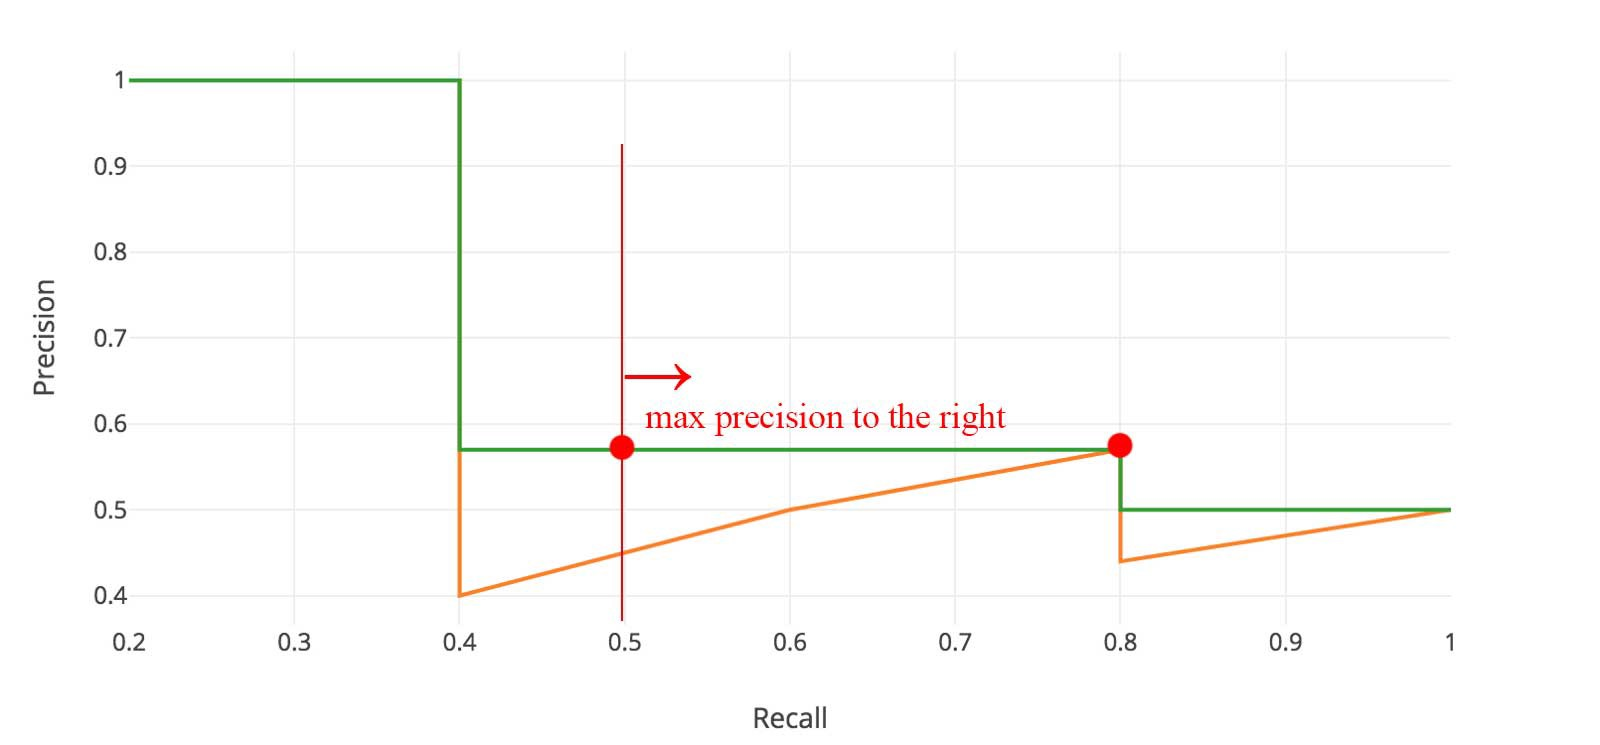
\includegraphics[width=7.5cm]{Bilder/map_graph1.png}} 
	\subfigure{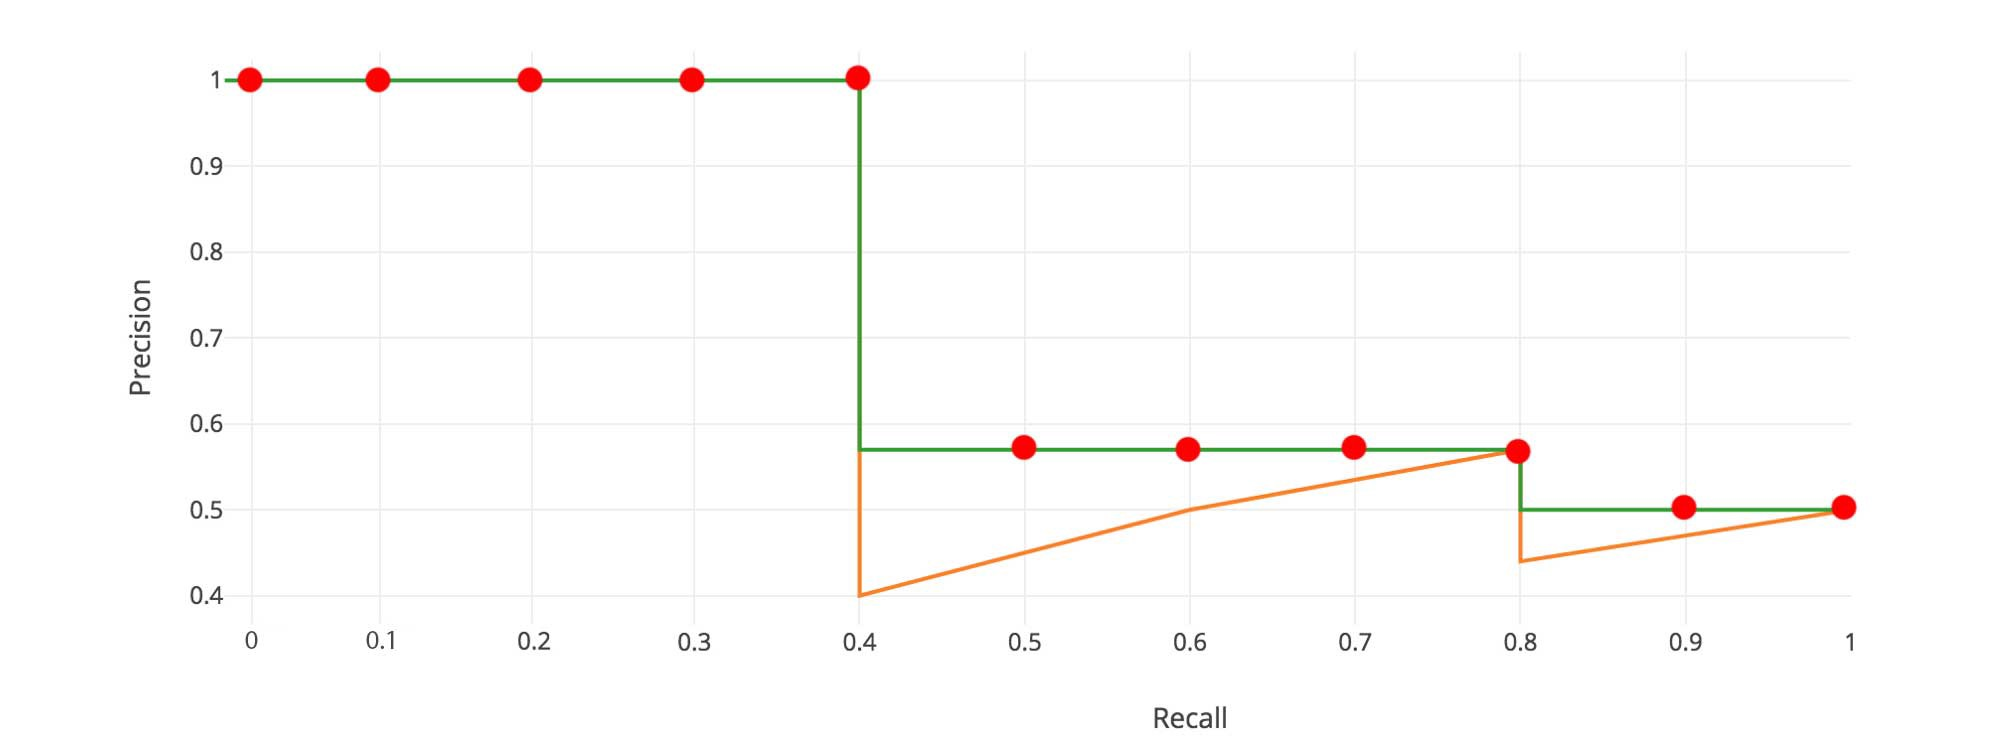
\includegraphics[width=7.5cm]{Bilder/map_graph2.png}} 
	\caption[Berechnung mAP]{Berechnung mAP \cite{JonathanHui.20180307}} 
	\label{map}
\end{figure} 

Im Graphen ist meist ein klassisches \glqq Zick-Zack\grqq{} Muster zu erkennen (siehe Abbildung \ref{map}). Dieses Muster wird geglättet, indem nach jedem Einbruch für jeden \textit{Recall} Wert der maximale \textit{Precision} Wert nach rechts übernommen wird. Bildet man anschließend das diskrete Integral, so ergibt sich der \textit{Average Precision} Wert für eine zu klassifizierende Kategorie. Der Mittelwert der  \textit{Average Precisions} über alle kategorien hinweg ergibt letztendlich den \textit{mAP} Wert \cite{JonathanHui.20180307}. 

\subsection*{Reaktionsvermögen}

FPS

\subsection*{Trainingsverhalten}


\subsection*{Interaktionsverhalten}

beleuchtung, doppelte erkennung

